\documentclass{manual}

\title{Getting Started with CoaSim/GUI}
\subtitle{An introduction to the simulator CoaSim}
\authors{Thomas Mailund}
\contact{mailund@birc.au.dk}
\company{Bioinformatics ApS}
\toolversion{CoaSim/GUI v3.1}

\usepackage{wrapfig}

\begin{document}

\section{About CoaSim}

CoaSim is a tool for simulating the coalescent process with
recombination and geneconversion, under either constant population
size or exponential population growth.  It effectively constructs the
ancestral recombination graph for a given number of chromosomes and
uses this to simulate samples of SNP and micro-satellite haplotypes or
genotypes.

CoaSim comes in two flavours: A graphical user interface version for
easy use by novice users, and a scripting based version (using either
Guile-Scheme or Python) for efficient batch simulations.  This
document is an introduction to the GUI version.

\subsection{Installing CoaSim}

CoaSim is distributed as RPM files or as source code.  For most users,
we recommend installing from the RPM files, since building the tool
from source requires setting up the right build environment and having
access to the needed development tools.  If you are not familiar with
UNIX C++ development---using the Automake suite of tools---and with Qt
development we do not recommend that you try building from source.

\paragraph{Installing the RPM Files.}

The RPM file, \verb?coasim-gui-x.y.z-r.i386.rpm?,  contains a binary
version of the program, compiled to an Intel x86 Linux platform.  To
install the graphical user interface version from the RPM package, run
\begin{code}
> rpm -Uvh coasim-gui-x.y.z-r.i386.rpm
\end{code}
where \texttt{x.y.z-r} is the version number of CoaSim.
Since the RPM files installs in the directory \verb?/usr/local/?,
installing the RPM package requires root access.

\paragraph{Installing from the Source Files.}

The source code is distributed in two tar-files:
\begin{itemize}
\item \verb?coasim-core-x.y.z.tar.gz?, and
\item \verb?coasim-gui-x.y.z.tar.gz?.
\end{itemize}

To build the source files, first untar the core module and place it in
a directory called Core:

\begin{code}
> tar zxf coasim-core-x.y.z.tar.gz
> mv coasim-core-x.y.z Core
> cd Core
> ./configure
> make
\end{code}

To build the graphical user interface to this simulation core, untar
the GUI source files next to the Core module, install the designer
plugins used, then qmake and build:

\begin{code}
> cd ..
> tar zxf coasim-gui-x.y.z.tar.gz
> cd coasim-gui-x.y.z/designer_plugins
> qmake
> make install
> cd ..
> qmake
> make
> make install
\end{code}

If you do not have write access to \verb?QTDIR/plugins?, you will need
to install the plugins locally, e.g. use qtconfig to add
\verb?$(HOME)/.qt/plugins? to the plugin path and do:

\begin{code}
> cd ..
> tar zxf coasim-gui-x.y.z.tar.gz
> cd coasim-gui-x.y.z/designer_plugins
> qmake
> INSTALL_ROOT=~/.qt make install
> cd ..
> qmake
> make
> make install
\end{code}


\subsection{Running CoaSim}

Installing the graphical user installing version should, on GNOME or
KDE desktops, add an icon in the start menu for running CoaSim.  If
this is not the case, the tool can be started on the command-line with
the command
\begin{code}
> coasim_gui
\end{code}

\section{Using CoaSim}

Running CoaSim will in most cases consist of three steps: Set up the
simulation parameters, including the markers (type of marker, mutation
rates and similar), demographic parameters, rates for recombination,
etc.; running the simulation obtaining and ARG; and extracting the
needed information from the ARG (\emph{Ancestral Recombination
  Graph}), e.g. the resulting sequences, the timing of the various
events, or the local coalescent trees embedded in the ARG.

The graphical user interface for CoaSim makes it possible for the
casual user to perform simple simulations; for more advanced use the
scripting facilities of the Scheme or Python based versions are needed.

In future releases we plan to build more power into the GUI version,
but at this moment limited resources forces us to focus our efforts on
one of the versions, and therefore the GUI version is limited compared
to the Guile Scheme version.

\begin{wrapfigure}{r}{5cm}
  \centering
  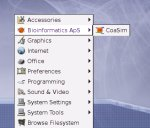
\includegraphics{figs/coasim-menu}
  \caption{The CoaSim icon in the menu.}
  \label{fig:menu}
\end{wrapfigure}
%%
Once CoaSim has been install, on most platforms it will appear in the
menu, as shown in Fig.~\ref{fig:menu}.  If it does not, however, it
can be started from the command line as
\begin{code}
> coasim_gui
\end{code}

Once started, the main window, shown on Fig.~\ref{fig:main}, appears.
This window is used to specify the markers to use in a simulation.
Using the tabs, different kinds of markers can be specified: trait
markers, used for specifying a trait of interest; SNP markers, similar
to trait markers, but with a different ascertainment bias; and
micro-satellite markers, with a different mutation model than the
other two.  Additional parameters for the simulation can be set in the
\emph{ARG Simulation Parameters} dialogue, shown in
Fig.~\ref{fig:arg-parameters}, opened from the \emph{Simulation} menu
in the main window.

\begin{figure}[tp]
  \centering
  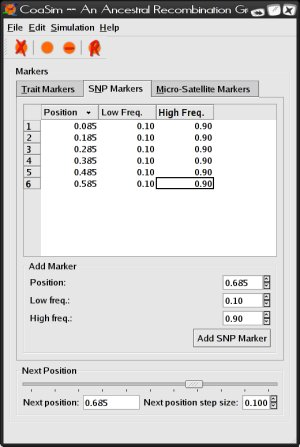
\includegraphics{figs/main-window}
  \caption{The CoaSim main window.  Used to set up markers for simulation.}
  \label{fig:main}
\end{figure}

\begin{figure}[tp]
  \centering
  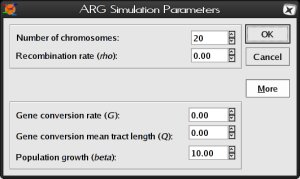
\includegraphics{figs/arg-parameters}
  \caption{Dialogue for setting ARG simulation parameters.}
  \label{fig:arg-parameters}
\end{figure}

Once the parameters have been set, the simulation can be started from
the \emph{Simulation} menu.  This opens the simulation monitor, shown
in Fig.~\ref{fig:monitor} and runs the simulation.  Once the
simulation has completed, the result is shown in the result dialogue
shown in Fig.~\ref{fig:results}.  From this dialogue it is possible to
save the result as a simple text file.

\begin{figure}[tp]
  \centering
  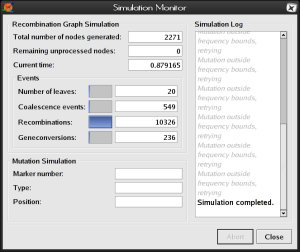
\includegraphics{figs/monitor}
  \caption{Simulation monitor, showing the progress of the monitor and
  different statistics about the simulation.}
  \label{fig:monitor}
\end{figure}

\begin{figure}[tp]
  \centering
  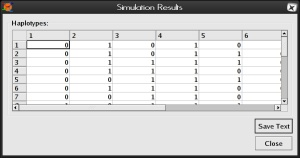
\includegraphics{figs/results}
  \caption{Simulation results.}
  \label{fig:results}
\end{figure}

\section{Contact}
\label{sec:contact}

For any comments or questions regarding CoaSim, please contact Thomas
Mailund, at \href{mailto:mailund@mailund.dk}{mailund@mailund.dk} or
\href{mailund@birc.au.dk}{mailund@birc.au.dk}.


\end{document}

% LocalWords:   CoaSim geneconversion haplotype haplotypes
